\documentclass{beamer}
\usepackage{amsmath}
\usepackage{amssymb}
\usepackage{amsfonts}
%\usepackage{graphics}
%\usepackage{curves}
\usepackage{tikz}
%\usetikzlibrary{backgrounds}
%\usetikzlibrary{snakes} 
%\usepackage{amsmath}
%\usepackage{amssymb}
%\usepackage{amsfonts}
%\usepackage{graphics}
%\usepackage{curves}
%\usepackage{tikz}
%\usetikzlibrary{backgrounds}
%\usetikzlibrary{snakes}
%\usepackage{setspace}
%\doublespacing
%\usepackage{lscape}
%\usepackage{booktabs}
%\usepackage{longtable}
\usepackage[normalem]{ulem}
\usepackage{hyperref}
\usepackage{url}
\usepackage{color}
\usepackage{bibentry}
\usepackage{graphicx}
%\nobibliography*
\bibliographystyle{plain}
\graphicspath{ {./figures/} }
\mode<presentation>
{
  \usetheme{default}      % or try Darmstadt, Madrid, Warsaw, ...
  \usecolortheme{default} % or try albatross, beaver, crane, ...
  \usefonttheme{default}  % or try serif, structurebold, ...
  \setbeamertemplate{navigation symbols}{}
  \setbeamertemplate{caption}[numbered]
} 

\usepackage[english]{babel}
\usepackage[utf8x]{inputenc}

\beamertemplatenavigationsymbolsempty

\setbeamerfont{page number in head/foot}{size=\small}
\setbeamertemplate{footline}[frame number]

\title[Your Short Title]{Wealth dynamics in the presence of network structure and primitive cooperation}
\author[shortname]{Rajesh Venkatachalapathy \inst{1} \and Stephen Davies \inst{2} \and William Nehrboss \inst{3}}
\institute[shortinst]{\inst{1} Systems Science Graduate Program \\Portland State University \\Portland, Oregon \and \inst{2} Department of Computer Science\\University of Mary Washington\\Fredericksburg, Virginia \and \inst{3} Lake Anna Homeschool\\Bumpass, Virginia}

%\author{Rajesh Venkatachalapathy}
%\institute{Systems Science Graduate Program \\Portland State University \\Portland, Oregon}
%
%
%
%\author{Stephen Davies}
%\institute{Systems Science Graduate Program \\Portland State University \\Portland, Oregon}
%\date{Friday 15th February 2019}




\begin{document}

\begin{frame}
\titlepage
\end{frame}


\begin{frame}[t]
\frametitle{Outline}
\begin{itemize}
\item Motivation and questions
\item Model
\item Experiments 
\item Findings 
\item Future work 
\end{itemize}
\end{frame}

\begin{frame}[t]
\frametitle{Motivation}
\begin{itemize}
\item Friesen-Mudigonda (FM) model 
\end{itemize}
Questions
\begin{itemize}
\item What is the social network analog of FM model?
\item What is the mathematical analog of ABM-based FM model? 
\item Do social structures mediate wealth accumulation? 
\item Does cooperation lead to more wealth?
\item Does cooperation improve chances of survival under resource scarcity?
\end{itemize}
\end{frame}

\begin{frame}[t]
\frametitle{Model}
FM model
\begin{itemize}
\item Agent-based model 
\item Resources are distributed in a grid world 
\item Agents interact as they forage for resources in \textit{this} grid world
\item  \textit{Wealthy enough} agents decide to pool their resources  
\end{itemize}
Our model 
\begin{itemize}
\item Stochastic dynamical system 
\item Resources are provided to each individual agent in a \textit{noisy manner}
\item Agents interact with neighbors in a static social network
\item \textit{Wealthy enough} agents decide to pool their resources 
\end{itemize}
\end{frame}

\begin{frame}[t]
\frametitle{Model}

Dynamics
\begin{equation}\label{ddm}
dx(t) = vdt + \sqrt{2D} dw
\end{equation}

\begin{itemize}
\item $v$ is the wealth growth rate (the difference of the income and metabolic rate of the agent) and $D$ is the intensity of the Brownian process (white noise process) $w$. 
\item $x(t)$ is the state of the particle (wealth) at time $t$. 
\item The dynamics can be started at any initial point $x_0 > 0$. 
\end{itemize}
Structure
\begin{itemize}
\item Erd\H{o}s-R\'{e}nyi network (ER) models
\end{itemize}
\end{frame}

\begin{frame}[t]
\frametitle{Vocabulary}
\begin{itemize}
\item proto
\end{itemize}
\end{frame}

\begin{frame}[t]
\frametitle{Experiments}
There are three \textbf{stages} in our experiments
\begin{itemize}
\item \textbf{Stage 1} is the phase of the dynamical model \textit{before} which any agents have formed protos
\item \textbf{Stage 2} is the phase \textit{during} which agents are formation protos.
\item \textbf{Stage 3} is the phase where all agents undergo starvation\footnote{This stage commences once all non-isiolate agents have jointed a proto.} 
\end{itemize}
\end{frame}

\begin{frame}[t]
\frametitle{Figures}
\begin{figure}[hb]
\centering
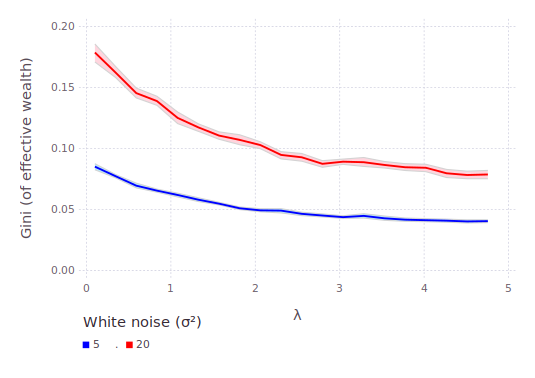
\includegraphics[scale=.4]{figures/giniVsLambda.png}
\caption{The average Gini coefficient of effective wealth (computed pre-Stage 3) for various values of the ER $\lambda$ connectivity parameter, and with both low-noise and high-noise income. 500 agents were used in each simulation. The color band represents a bootstrapped 95\% confidence interval.}
\label{fig:giniVsLambda}
\end{figure}
\end{frame}

\begin{frame}[t]
\frametitle{Figures}
\begin{figure}[ht]
\centering
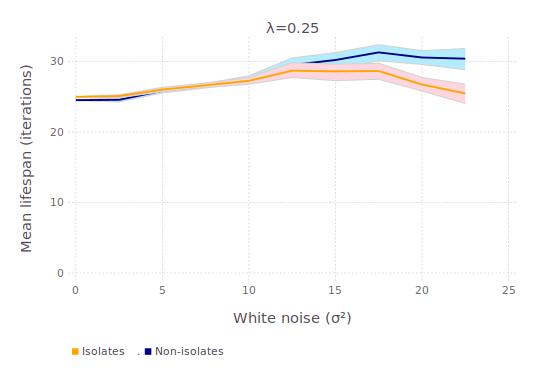
\includegraphics[scale=.4]{figures/avgLifespanLambda_025.png}
\caption{Life expectancy comparison between isolates (non-proto members) and
non-isolates (proto members) for different values of $\lambda$ and $\sigma^2$.
The \texttt{salary} parameter was set to 20, so the x-axis ranges from a nearly
constant agent income to a scenario when the noise is as high as the average.}
\label{fig:avgLifespanLambda}
\end{figure}
\end{frame}

\begin{frame}[t]
\frametitle{Figures}
\begin{figure}[ht]
\centering
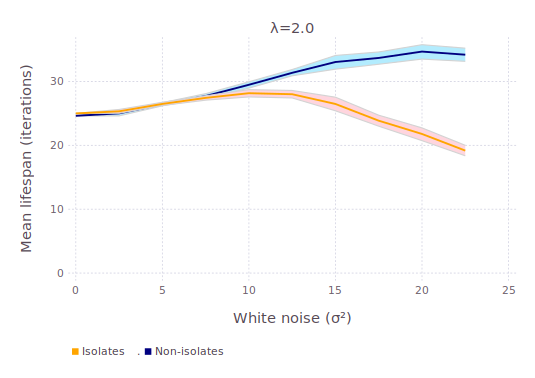
\includegraphics[scale=.4]{figures/avgLifespanLambda2.png}
\caption{Life expectancy comparison between isolates (non-proto members) and
non-isolates (proto members) for different values of $\lambda$ and $\sigma^2$.
The \texttt{salary} parameter was set to 20, so the x-axis ranges from a nearly
constant agent income to a scenario when the noise is as high as the average.}
\label{fig:avgLifespanLambda}
\end{figure}
\end{frame}

\begin{frame}[t]
\frametitle{Results}
%% need to link the figures here 
\begin{itemize}
\item Larger environmental noise produces large inequality measures (Figure 1)
\item Larger the noise, larger the separation between the mean lifetimes of the two populations (Figures 2 and 3) 
\item Larger connectivity leads to a more egalitarian population
\item Larger connectivity leads to larger separation between the mean lifetimes of the two populations
\end{itemize}

\end{frame}

\begin{frame}[t]
\frametitle{Questions}
\begin{itemize}
\item What are the underlying mechanisms underlying the gap between mean life expectancy of \textit{protos} and \textit{isolates}?
\item Do \textit{protos} of different sizes differ in the mean life expectancy and wealth? 
\item Can we derive the results of these simulations from the defining SDS?
\item Do other baseline network models like \textit{scale-free} and \textit{small-world} models induce similar systematic differences between \textit{protos} and \textit{isolates}?
\end{itemize}
\end{frame}

\begin{frame}[t]
\frametitle{Conclusion}
\begin{itemize}
\item These are very preliminary results 
\item Repeating these simulations on other baseline network models might provide more clarity
\item These models might be amenable to mean field analysis 
\end{itemize}
More generally
\begin{itemize}
\item Our models are an useful addition to the variety of dynamical system models on networks 
\item Despite their simplicity, the exhibit interesting dynamics and are useful to study the two-way interaction between structure and dynamics.  
\end{itemize}
\end{frame}

\end{document}